    \documentclass{llncs}

% Propositional rules
\newcommand{\lr}{\mf L}
\newcommand{\rr}{\mf R}
\newcommand{\lbot}{$\bot_\lr$}
\newcommand{\rtop}{$\top_\rr$}
\newcommand{\lto}{$\to_\lr$}
\newcommand{\rto}{$\to_\rr$}
\newcommand{\init}{$\mf{init}$}
\newcommand{\lland}{$\land_\lr$}
\newcommand{\rland}{$\land_\rr$}

% Modal rules
\newcommand{\lbox}{$\Box_\lr$}
\newcommand{\rbox}{$\Box_\rr$}
\newcommand{\rboxm}{${}_{\mathsf M}\Box_\rr$}


%ANNOTATED RULES
% Propositional rules
\newcommand{\lrA}{\mf L}
\newcommand{\rrA}{\mf R}
\newcommand{\lbotA}{$\bot_\lr^{\annotated}$}
\newcommand{\rtopA}{$\top_\rr^{\annotated}$}
\newcommand{\ltoA}{$\to_\lr^{\annotated}$}
\newcommand{\rtoA}{$\to_\rr^{\annotated}$}
\newcommand{\initA}{$\mf{init}^{\annotated}$}

% Modal rules
\newcommand{\lboxA}{$\Box_\lr^{\annotated}$}
\newcommand{\rboxA}{$\Box_\rr^{\annotated}$}
\newcommand{\rboxmA}{${}_{\mathsf M}\Box_\rr^{\annotated}$}
\newcommand{\rulenA}{$\mf N^{\annotated}$}
\newcommand{\rulecA}{$\mf C^{\annotated}$}


\newcommand{\rboxc}{$\Box_\textup{R}^\textup{C}$}
\newcommand{\rulen}{$\mf N$}
\newcommand{\rulem}{$\Box_\textup{R}^\textup{M}$}
\newcommand{\rboxmc}{$\Box_\textup{R}^\textup{MC}$}
\newcommand{\rulec}{$\mf C$}
\newcommand{\rulep}{$\mf P$}
\newcommand{\rulet}{$\mf T$}
\newcommand{\ruled}{$\mf D$}
\newcommand{\ruledm}{$\mf D_{\mathsf M}$}
\newcommand{\ruledaux}{$\mf D_{\mathsf{aux}}$}


\newcommand{\mc}{\mathcal}
\newcommand{\mf}{\mathsf}
\newcommand{\tbf}{\textbf}
\newcommand{\mbf}{\mathbf}

% classical non-normal modal logics
\newcommand{\Logic}{$\mathbf{L}$}
\newcommand{\Logicstar}{$\mathbf{L^{\star}}$} 
\newcommand{\Estar}{$\mathbf{E^{\star}}$}  
\newcommand{\E}{$\mathbf{E}$}
\newcommand{\EM}{$\mathbf{M}$}
\newcommand{\EN}{$\mathbf{EN}$}
\newcommand{\EC}{$\mathbf{EC}$}
\newcommand{\EMN}{$\mathbf{MN}$}
\newcommand{\ECN}{$\mathbf{ECN}$}
\newcommand{\EMC}{$\mathbf{MC}$}
\newcommand{\EMCN}{$\mathbf{MCN}$}

\newcommand{\K}{$\mathbf{K}$}

\newcommand{\EMD}{$\mathbf{MD}$}
\newcommand{\Eextstar}{$\mathbf{E(T/P/D)^{\star}}$}  

\newcommand{\CPL}{$\mathbf{PL}$}


\newcommand{\mathET}{\mathbf{ET}}
\newcommand{\mathEMD}{\mathbf{MD}}
\newcommand{\mathEND}{\mathbf{END}}
\newcommand{\mathECP}{\mathbf{ECP}}



% Axioms
\newcommand{\axMdiam}{$\mathsf M_\Diamond$}
\newcommand{\axCdiam}{$\mathsf C_\Diamond$}
\newcommand{\axNdiam}{$\mathsf N_\Diamond$}
\newcommand{\axMbox}{$\mathsf M_\Box$}
\newcommand{\axCbox}{$\mathsf C_\Box$}
\newcommand{\axNbox}{$\mathsf N_\Box$}
\newcommand{\dualbox}{$\mathsf{Dual_\Box}$}
\newcommand{\dualdiam}{$\mathsf{Dual_\Diamond}$}
\newcommand{\axKdiam}{$\mathsf K_\Diamond$}
\newcommand{\MP}{$\mathsf{MP}$}



%rules names
\newcommand{\rebox}{$\mathsf{RE_\Box}$}
\newcommand{\rediam}{$\mathsf{RE_\Diamond}$}
\newcommand{\rmbox}{$\mathsf{RM_\Box}$}
\newcommand{\rmdiam}{$\mathsf{RM_\Diamond}$}
\newcommand{\rulenbox}{$\mathsf{RN_\Box}$}
\newcommand{\rulendiam}{$\mathsf{RN_\Diamond}$}


\newcommand{\ax}{\AxiomC}
\newcommand{\uinf}{\UnaryInfC}
\newcommand{\binf}{\BinaryInfC}
\newcommand{\llab}{\LeftLabel}
\newcommand{\rlab}{\RightLabel}
\newcommand{\disp}{\DisplayProof}
%\newcommand{\seq}{\vdash}
\newcommand{\seq}{\Rightarrow}
%\newcommand{\hyp}{\parallel}
\newcommand{\hyp}{\mid}
\newcommand{\G}{\Gamma}
\newcommand{\D}{\Delta}
%\newcommand{\boxes}{\langle\Lambda\rangle}
\newcommand{\boxes}{\Lambda^{\langle \rangle}}
%\newcommand{\boxes}{{}_{\langle \rangle}\Lambda}
%\newcommand{\hG}{\mathfrak G}
%\newcommand{\hD}{\mathfrak D}
%\newcommand{\hG}{\mathcal G}
%\newcommand{\hD}{\mathcal D}
\newcommand{\hG}{G}
\newcommand{\hD}{D}
\newcommand{\hH}{H}







%Model
\newcommand{\Pow}{\mc P}
\newcommand{\M}{\mc M}
\newcommand{\Ms}{\mc M_s}
\newcommand{\N}{\mc N}
\newcommand{\Ns}{\mc N_s}
\newcommand{\Nb}{\mc N_b}
\newcommand{\W}{\mc W}
\newcommand{\V}{\mc V}
%\newcommand{\mod}{\models}
\newcommand{\Vd}{\Vdash}
\newcommand{\vd}{\vdash}
\newcommand{\B}{\mc B}
\newcommand{\C}{\mc C}

\newcommand{\Der}{\mathcal D}
\newcommand{\DerA}{\mathcal D^*}

\newcommand{\lan}{\mc L}
\newcommand{\atm}{\mf{Atm}}
\newcommand{\s}{\mc S}

%\newcommand{\tsets}[1]{[#1]_{\M}^s}
%\newcommand{\tsetb}[1]{[#1]_{\M}^b}
\newcommand{\tsets}[1]{[#1]_{\M}}
\newcommand{\tsetb}[1]{[#1]_{\M}}

% Annotated calculus
\newcommand{\AB}{\mathcal A}
%\newcommand{\AB}{\mathsf{A}_{\B}}
%\newcommand{\AB}{\mathsf{A}}
\newcommand{\annotation}{(\aw, \af, \apol)}
\newcommand{\inann}{(x_0, \epsilon, \epsilon)}
\newcommand{\inannone}{(x_1, \epsilon, \epsilon)}
\newcommand{\inannn}{(x_n, \epsilon, \epsilon)}
%\newcommand{\annotated}{\A}
\newcommand{\annotated}{*}
\newcommand{\aw}{x}
\newcommand{\af}{\phi}
\newcommand{\apol}{\circ}
\newcommand{\roothyp}{\G_1 \seq^{\inannone} \D_1 \hyp ... \hyp \G_n \seq^{\inannn} \D_n}

%
\newcommand{\HL}{$\mc H_{\mathsf L}$}
\newcommand{\HE}{$\mc H_{\mathsf E}$}
\newcommand{\HM}{$\mc H_{\mathsf M}$}
\newcommand{\HEC}{$\mc H_{\mathsf{EC}}$}
\newcommand{\HMC}{$\mc H_{\mathsf{MC}}$}
\newcommand{\HEN}{$\mc H_{\mathsf{EN}}$}
\newcommand{\HMN}{$\mc H_{\mathsf{MN}}$}
\newcommand{\HECN}{$\mc H_{\mathsf{ECN}}$}
\newcommand{\HMCN}{$\mc H_{\mathsf{MCN}}$}
%\newcommand{\HEMCN}{$\mc H_{\mathsf{E(M,C,N)}}$}
\newcommand{\HEMCN}{$\mc H_{\mathsf{E(M/C/N)}}$}
\newcommand{\HEMCNext}{$\mc H_{\mathsf{E(M/C/N/T/P/D)}}$}

\newcommand{\HEstar}{$\mc H_{\mathsf E^{\star}}$}
\newcommand{\HMstar}{$\mc H_{\mathsf M^{\star}}$}
\newcommand{\HENstar}{$\mc H_{\mathsf{EN}^{\star}}$}
\newcommand{\HECstar}{$\mc H_{\mathsf{EC}^{\star}}$}
\newcommand{\HEextstar}{$\mc H_{\mathsf{E(T/P/D)}^{\star}}$}

\newcommand{\aHE}{$\mc H_{\mathsf E}^{*}$}
\newcommand{\aHM}{$\mc H_{\mathsf M}^{*}$}
\newcommand{\aHEC}{$\mc H_{\mathsf{EC}}^{*}$}
\newcommand{\aHMC}{$\mc H_{\mathsf{MC}}^{*}$}
\newcommand{\aHEN}{$\mc H_{\mathsf{EN}}^{*}$}
\newcommand{\aHMN}{$\mc H_{\mathsf{MN}}^{*}$}
\newcommand{\aHECN}{$\mc H_{\mathsf{ECN}}^{*}$}
\newcommand{\aHMCN}{$\mc H_{\mathsf{MCN}}^{*}$}
\newcommand{\aHEMCN}{$\mc H_{\mathsf{E(M,C,N)}}^{*}$}

\newcommand{\aHEstar}{$\mc H_{\mathsf E^{\star}}^{*}$}
\newcommand{\aHMstar}{$\mc H_{\mathsf M^{\star}}^{*}$}
\newcommand{\aHENstar}{$\mc H_{\mathsf{EN}^{\star}}^{*}$}
\newcommand{\aHECstar}{$\mc H_{\mathsf{EC}^{\star}}^{*}$}


\newcommand{\bH}{$H$$\downarrow$}


% Hilbert Axioms
\newcommand{\axM}{$\textup M$}
\newcommand{\axN}{$\textup N$}
\newcommand{\axC}{$\textup C$}
\newcommand{\axK}{$\textup K$}
\newcommand{\axP}{$\textup P$}
\newcommand{\axD}{$\textup D$}
\newcommand{\axT}{$\textup T$}
\newcommand{\RE}{$\textup{RE}$}
\newcommand{\RM}{$\textup{RM}$}
\newcommand{\RN}{$\textup{RN}$}
%\newcommand{\axM}{$\mf M$}
%\newcommand{\axN}{$\mf N$}
%\newcommand{\axC}{$\mf C$}
%\newcommand{\axK}{$\mf K$}
%\newcommand{\axP}{$\mf P$}
%\newcommand{\axD}{$\mf D$}
%\newcommand{\RE}{$\mf{RE}$}
%\newcommand{\RM}{$\mf{RM}$}
%\newcommand{\RN}{$\mf{RN}$}


% B: Note you don't need those if you use the last command \str with an
% argument :)  T: Thank you B. I read your comment too late. 
\newcommand{\angA}{\langle A \rangle}
\newcommand{\angB}{\langle B \rangle}
\newcommand{\angC}{\langle C \rangle}
\newcommand{\angtop}{\langle \top \rangle}
\newcommand{\angSigma}{\langle \Sigma \rangle}
\newcommand{\angPi}{\langle \Pi \rangle}
\newcommand{\angLambda}{\langle \Lambda \rangle}
\newcommand{\angTheta}{\langle \Theta \rangle}
\newcommand{\angXi}{\langle \Xi \rangle}
\newcommand{\angUpsilon}{\langle \Upsilon \rangle}
\newcommand{\angOmega}{\langle \Omega \rangle}
\newcommand{\angSigmaPi}{\langle \Sigma, \Pi \rangle}
\newcommand{\str}[1]{\langle #1 \rangle}

\newcommand{\set}[1]{\mathsf{set}(#1)}
\newcommand{\HC}[1]{\mathcal{H}_{#1}}
\newcommand{\logic}{\mathbf{L}}

% Structural rules
\newcommand{\wk}{$\mathsf{wk}$}
\newcommand{\ctr}{$\mathsf{ctr}$}  
\newcommand{\lwk}{$\mathsf{wk_\lr}$}
\newcommand{\rwk}{$\mathsf{wk_\rr}$}
\newcommand{\lctr}{$\mathsf{ctr_\lr}$}
\newcommand{\rctr}{$\mathsf{ctr_\rr}$}
%\newcommand{\angwk}{$\mathsf{wk_{<>}}$}  
%\newcommand{\angctr}{$\mathsf{ctr_{<>}}$} 
\newcommand{\angwk}{$\mathsf{wk_{\langle\rangle}}$}  
\newcommand{\angctr}{$\mathsf{ctr_{\langle\rangle}}$} 


\newcommand{\exex}{$\mathsf{ee}$}  
\newcommand{\intctr}{$\mathsf{ctr}$}
\newcommand{\exctr}{$\mathsf{ec}$}    
\newcommand{\intwk}{$\mathsf{wk}$}
\newcommand{\exwk}{$\mathsf{ew}$}
\newcommand{\hypcut}{$\mathsf{cut}$}
\newcommand{\subrule}{$\mathsf{sub}$}
\newcommand{\subrulem}{$\mathsf{sub_M}$}
\newcommand{\subruleaux}{$\mathsf{sub_{(M)}}$}

\newcommand{\cllogic}{classical non-normal modal logic}
\newcommand{\bin}{bi-neighbourhood}
\newcommand{\nei}{neighbourhood}
\newcommand{\Angle}{block}
\newcommand{\AND}{\bigwedge}
\newcommand{\OR}{\bigvee}
\newcommand{\fint}{i}
\newcommand{\w}{\mf w}
\newcommand{\sbf}{\mf{sbf}}

\newcommand{\nann}{\mathbf a}
\newcommand{\nbl}{\mathbf b}
\newcommand{\sizebl}{\mathbf{sb}}

%%% SIDE COMMENTS ENVIRONMENT

\newcommand{\nb}[1]{\textcolor{red}{$|$}\mbox{}\marginpar{\scriptsize\raggedright\textcolor{red}{#1}}}

\newcommand{\hide}[1]{}

% prints the text only in the appropriate version
% requires etoolbox package
\newcommand{\inVersion}[2]{\ifdefstring{\versionlength}{#1}{#2}{
\ifdefstring{\versionlength}{all}{\noindent \textbf{In #1 Version: }
  #2 \textbf{End of  #1 Version}\\}{}
}}

% General purpose macros
\newcommand\eg{\hbox{\textit{e.g.}}}
\newcommand\ie{\hbox{\textit{i.e.}}}
\newcommand{\etal}{\emph{et al.}}
\newcommand{\red}[1]{\textcolor{red}{#1}}
\newcommand{\blue}[1]{{\color{blue}{#1}}}

\newenvironment{proof-sketch}{\noindent{\em Sketch of Proof.}\hspace*{0.5em}}{\qed\medskip}%{\qed\medskip}%{\qed\bigskip}

\newcommand\blfootnote[1]{%
  \begingroup
  \renewcommand\thefootnote{}\footnote{#1}%
  \addtocounter{footnote}{-1}%
  \endgroup
}

\newcommand{\cyan}[1]{\textcolor{cyan}{#1}}

%TODO notes
%\renewcommand{\note}[3]{\todo[size=\tiny,color=#1]{\texttt{\color{white} #2: #3}}}
%\newcommand\co[1]{\note{orange}{CO}{#1}}
%\newcommand\ep[1]{\note{blue}{EP}{#1}}
%\newcommand\rl[1]{\note{green}{\color{black}RL}{\color{black}#1}}
%\newcommand\review[1]{\note{yellow}{\color{black}}{\color{black}#1}}
%\newcommand\reviewin[1]{\note{yellow,inline}{\color{black}}{\color{black}#1}}
%\newcommand\warning[1]{\note{red}{ACHTUNG!}{#1}}

%%% 
\usepackage[utf8]{inputenc}
\usepackage[T1]{fontenc}
\usepackage{epigraph}
\usepackage{lettrine}
\usepackage{type1ec}
\usepackage{latexsym}
%\usepackage{amsmath}
\usepackage[makeroom]{cancel}
%\usepackage{amsfonts}
\usepackage{amssymb}
%\usepackage{amsthm}
%\usepackage{mathrsfs}
\usepackage{setspace}
\usepackage{afterpage}
\usepackage{newlfont}
\usepackage{array}
\usepackage{tabularx}
\usepackage{dcolumn}
\usepackage{etoolbox}

\usepackage[hide]{ed}
\usepackage{graphicx}
\usepackage[misc]{ifsym}

%\usepackage{booktabs}
\usepackage[bf]{caption}
\usepackage{tikz}
\usepackage{xcolor}
\usepackage{color}
\usetikzlibrary{arrows}
%\usepackage{IEEEtrantools}
\usepackage{bussproofs}
\usepackage{proof}
\usepackage[lined,linesnumbered,algoruled]{algorithm2e}
%\usepackage{stmaryrd}
\usepackage{multirow}

%\usepackage{todonotes}
\usepackage{lmodern}

\title{Semantic tables for non-normal modal logics}
\author{DRAFT}
\date{August 2025}

\begin{document}

\maketitle

\section{Introduction}
Non-normal modal logics--NNMLs for short--have a long history, going back to the seminal works by Kripke, Montague, Segeberg, Scott, and Chellas (see 
\cite{Chellas:1980fk} for an introduction). They are ``non-normal'' as they do not contain all axioms of minimal \emph{normal} modal logic  \K. 

In this work, we consider  the {\em classical cube} on NMMLs, given by the extensions of the  minimal modal logic \E, containing only the {\em congruence rule}, 
with axioms \axC, \axM\ and \axN.


NNMLs have a well-understood semantics defined in terms of
neighbourhood models \cite{Pacuit:2017}: in these models  each world $w$ has an
associated set of neighbourhoods $\N(w)$, each one of them being a set
of worlds/states.  If we accept the traditional interpretation of a ``proposition'' as a set of worlds, we can think of  each neighbourhood  in $\N(w)$ as a proposition: a formula
$\Box A$ is true in a world $w$ if ``the proposition'' $A$, \ie\ the truth-set of $A$, belongs to
$\N(w)$.  The classical cube can be modelled by imposing additional closure properties of the set of neighbourhoods.  

%In~\cite{DBLP:conf/lfcs/DalmonteLOP20,DBLP:journals/logcom/DalmonteLOP21} we adopted a variant of neighbourhood semantics defined in terms of bi-neighbourhood models: in these structures each world has associated a set of \emph{pairs} of neighbourhoods. The intuition is that the two components of a pair provide positive and negative support for a modal formula, being more natural for ``non-monotonic'' logics (\ie\ not containing axiom \axM). The reason is that, instead of specifying exactly the truth sets in $\N(w)$, the pairs of neighbourhoods specify just lower and  upper bounds of truth sets, so that the same pair may be a ``witness'' for several propositions.  This makes the generation of \emph{countermodels} easier.

It is curious to note that, although some proof-systems for NNMLs have been proposed in the past, countermodel extraction has been rarely addressed and complexity is seldom analysed. We filled this gap in~\cite{DBLP:journals/logcom/DalmonteLOP21} by
proposing \emph{modular} 
calculi for the classical cube (and also some deontic extensions)  that provide  {\em direct countermodel extraction} 
and are of {\em optimal complexity}.  


In this work, we intend to have a semantic analysis of NNMLs using the so called RNMatrices.

\section{Non-normal modal logics}\label{sec:nnml}


In this section, we present  the classical cube of NNMLs, both axiomatically and semantically in terms of neighbourhood models. 
%We also present \bin{} models, a variant of the neighbourhood semantics introduced in \cite{Dalmonte:2018AIML}.

The propositional language $\lan$ contains \emph{formulas} given by the following grammar:
\[A ::= p  \mid \bot \mid A \to A \mid \Box A\]
where $p\in\at$, the set of propositional variable symbols. 
%
Other propositional connectives are defined by the standard equivalences.

The minimal  logic \E{} in the language $\lan$ is given Hilbert-style by extending classical propositional logic with only the \emph{congruence rule}
%
\begin{center}
\AxiomC{$A \to B$}
\AxiomC{$B \to A$}
\LeftLabel{\RE}
\BinaryInfC{$\Box A \to \Box B$}
\DisplayProof
\end{center}

The {\em classical cube} (below right) is formed by extending 
\E\ 
with any combination of axioms \axM, \axC{}, and \axN{}
(below left).

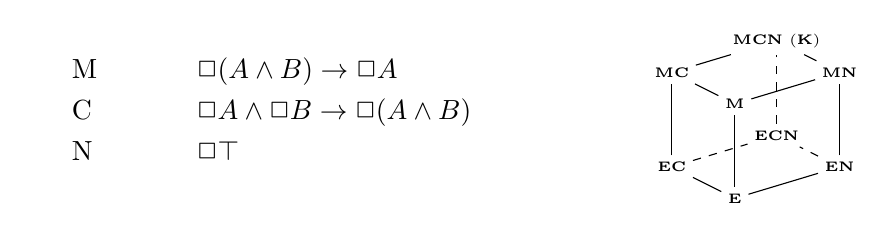
\begin{tikzpicture}
\node (AX) [label=90: {
\begin{tabular}{llll}
\vspace{0.1cm}
\axM &&& $\Box (A \land B)\to \Box A$ \\
\vspace{0.1cm}
\axC &&& $\Box A \land \Box B \to \Box (A \land B)$ \\
\vspace{0.1cm}
\axN &&& $\Box \top$
\end{tabular}}] at (-6,-0) {};
%
\begin{tiny}
	\node (a) at  (0,0)  {\E};
    \node (b) at (0, 1.2) {\EM};
    \node  (c) at (-0.8, 0.4) {\EC};
    \node (d) at (1.33, 0.4) {\EN};
    \node (e) at (-0.8, 1.6) {\EMC};
    \node (f) at (1.33, 1.6) {\EMN}; 
    \node (g) at (0.53, 0.8) {\ECN};
    \node (h) at (0.53, 2) {\EMCN{} (\K)};

\draw (a) -- (b);
\draw (a) -- (c);
\draw (a) -- (d);
\draw (b) -- (e);
\draw (b) -- (f);
\draw (c) -- (e);
\draw [dashed] (c) -- (g);
\draw (d) -- (f);
\draw [dashed] (d) -- (g);
\draw (e) -- (h);
\draw (f) -- (h);
\draw [dashed] (g) -- (h);
\end{tiny}
\end{tikzpicture}

As usual for logics containing \axM{} we omit \E,  \eg, we write \EMC{} for \textsf{EMC}.
%
In the following, for any system \Logic{} of the cube we denote with \Logicstar{} any extension of \Logic{} obtained by adding one or more of these axioms.

We recall that 
axioms \axM{} and \axN{}
are, respectively, equivalent
to the rules
\begin{prooftree}
\AxiomC{$A \to B$}
\LeftLabel{\RM}
\UnaryInfC{$\Box A \to \Box B$}
\DisplayProof
\qquad and \qquad
\AxiomC{$A $}
\LeftLabel{\RN}
\UnaryInfC{$\Box A$}
\end{prooftree}
and that axiom
\axK{} ($\Box (A \to B) \to \Box A \to \Box B$)
is derivable from \axM{} and \axC.
As a consequence,  
the top system \EMCN{}
is equivalent to \K,  the weakest normal modal logic.


The standard semantics for NNMLs is defined  in terms of so-called neighbourhood (or minimal) models~\cite{Chellas:1980fk}.    
\begin{definition}
A \emph{neighbourhood model} is a tuple $\M = \langle \W, \N, \V \rangle$, where $\W$ is a non-empty set,
$\V$ is a valuation function, and $N(w)$ is a neighbourhood function $\W \longrightarrow \Pow(\Pow(\W))$.
%
A model $\M$ 
\begin{itemize}
\item is \emph{monotone} if $\alpha\in\N(w)$ and
$\alpha\subseteq\beta\subseteq \W$ implies $\beta\in\N(w)$;
\item \emph{contains the emptyset} if $\varnothing\in\N(w)$; \emph{contains the unit} if $\W\in\N(w)$ for all $w\in\W$; 
\item is \emph{closed under intersection} if $\forall i \in I, \alpha_{i} \in \N(w) \Rightarrow \bigcap_{i \in I} \alpha_{i} \in \N(w)$. $\M$ is {\em closed under finite intersection} if $I$ is finite.
\item is \emph{closed under union} if $\forall i \in I, \alpha_{i} \in \N(w) \Rightarrow \bigcup_{i \in I} \alpha_{i} \in \N(w)$. %$\M$ is {\em closed under finite uniton} if $I$ is finite.
\item The set $\bigcap \N(w)$ is called the core of $\N(w)$; when $\bigcap \N(w)\in\N(w)$, $\N(w)$ is said to {\em contain its core}.
\end{itemize}
\end{definition}

Some of these neighborhood structures are well-known  in Mathematics. 

\begin{definition} Let $\W \neq \varnothing$ and $\N(w) \subseteq \mathcal{P}(\mathcal{P}(\W))$. We say that: 
\begin{itemize}
    \item $N(w)$ is a {\em topology} if $N(w)$ contains the empty set, the unit, and is closed under finite intersections and unions. 
    \item $N(w)$ is a {\em filter} if it contains the unit, is closed under finite intersection, and is monotonic; $N(w)$ is a {\em proper filter} if it is a filter and $\varnothing \notin \N$. 
    \item $N(w)$ is an {\em ultrafilter} if $N(w)$ is a proper filter and, furthermore, $\forall \alpha \subseteq \W \Rightarrow \alpha \in \N$ or $\alpha^{c} \in \N$. 
    \item $N(w)$ is {\em augmented} if $N(w)$ contains its core and is monotonic.
\end{itemize}
\end{definition}

\begin{definition}  Let $\mathcal{M} = (\W, \N, \V)$ be a neighborhood model, $w \in \W$. The forcing relation is defined as follows.
\begin{enumerate}
    \item $\mathcal{M}, w \Vdash p \Leftrightarrow w \in \V(p)$, if $p \in \at$
    \item $\mathcal{M}, w \not\Vdash \bot$ for any $w$ 
    \item $\mathcal{M}, w \Vdash A \rightarrow B \Leftrightarrow$ if $\mathcal{M}, w \Vdash \phi$ then $\mathcal{M}, w \Vdash \psi$ 
    \item $\mathcal{M}, w \Vdash \Box A \Leftrightarrow \tsets{A} \in N(w)$
\end{enumerate}
where $\tsets{A}$ denotes the set $\{v \in \W \mid \M, v \Vd A\}$ of the worlds $v$
that force $A$, also called the {\em truth set of $A$}. 
\end{definition} 
 
Neighbourhood models characterise modularly the classical cube of NNMLs \cite{Chellas:1980fk} in the sense that a formula $A$ is a theorem of  \E{} if and only if it is valid in all neighbourhood models.  
Furthermore, 
$A$ is a theorem of 
\E{}+(\axM /\axC /\axN) iff it is valid, respectively, in all  models that are monotonic (\axM),  closed under intersection (\axC), and contain the unit (\axN) (and any combination of these previous axioms/conditions). 

\begin{theorem}
The logics \E{} / \E{\axC}/ \E{\axN}/ \E{\axM} are sound and strongly complete with respect to the class of
\begin{itemize}
\item  all neighbourhood frames.
\item neighbourhood frames that are closed under intersections.
\item  neighborhood frames that contain the unit.
\item monotonic frames.
\end{itemize}
\end{theorem}


\begin{theorem}
\begin{itemize}
\item The class $K = \{\M | \M \mbox{ is a relational model} \}$ is modally equivalent to the class $\M_{aug} = \{\M | \M \mbox{ is an augmented neighborhood model}\}$.

\item The class $K^n = \{\M | \M \mbox{ is an n-ary relational model} \}$ is modally equivalent to the class $\M_{mon} =  \{\M | \M \mbox{ is a monotone neighborhood model}\}$.
\end{itemize}
\end{theorem}

The further axioms we
are going to consider are (using the terminology
of~\cite{Hansen:2003}):
\[
  \mathsf{P}\; \neg \Box \bot
  \qquad
  \mathsf{D}\; \neg (\Box A \land \Box \neg A)
  \qquad
  \mathsf{T}\; \Box A \to A
  \qquad
  \mathsf{4}\; \Box A \to \Box \Box A
  \qquad
  \mathsf{5}\; \Box A \lor \Box \neg \Box A
\]
Note that we included both the two axioms $\mathsf{P}$ and $\mathsf{D}$ which are
usually taken to be two different formulations of the seriality axiom. % for
% seriality.
This is due to the fact that in the non-normal setting the
two formulations are not equivalent: while $\mathsf{P}$ is derivable from
$\mathsf{D}$, the opposite does not hold in logics not validating the axiom
\axC. The reason for why we here only consider extensions of monotone
modal logic with these axioms instead of extensions of classical modal
logic $\mathsf{E}$ is that obtaining cut-free sequent calculi for many
of these extensions seems to be problematic~\cite{Indrzejczak:2011}.

The objective is to study all the logics in
what could be called the \emph{modal tesseract}
(Fig.~\ref{fig:modal-tesseract}), hence repairing the bridge between
non-normal and normal modal logics. Note that the modal tesseract
includes one side of the standard (normal) modal cube, see
e.g.~\cite{Brunnler:2009kx}.
\begin{figure}[t]
  \hrule\bigskip
  \begin{center}
    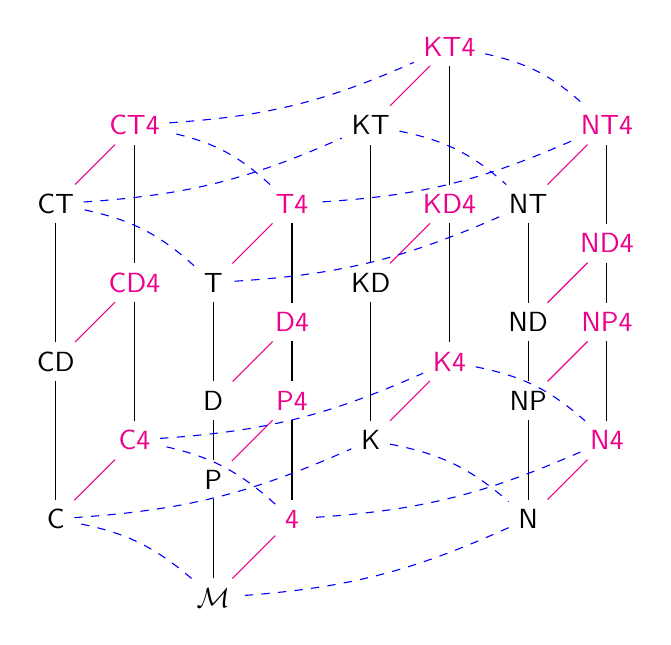
\begin{tikzpicture}
      \node (M) at (0,0) {$\M$};
      \node (MD1) at (0,1.5) {$\mathsf{P}$};
      \node (MD2) at (0,2.5) {$\mathsf{D}$};
      \node (MT) at (0,4) {$\mathsf{T}$};
      \node (M4) [color=magenta] at (1,1) {$\mathsf{4}$};
      \node (MD14) [color=magenta] at (1,2.5) {$\mathsf{P}\mathsf{4}$};
      \node (MD24) [color=magenta] at (1,3.5) {$\mathsf{D}\mathsf{4}$};
      \node (MT4) [color=magenta] at (1,5) {$\mathsf{T}\mathsf{4}$};
      \draw [color=magenta] (M) -- (M4);
      \draw [color=magenta] (MD1) -- (MD14);
      \draw [color=magenta] (MD2) -- (MD24);
      \draw [color=magenta] (MT) -- (MT4);
      \draw (M) -- (MD1) -- (MD2) -- (MT);
      \draw (M4) -- (MD14) -- (MD24) -- (MT4);
%%
      \node (C) at (-2,1) {$\mathsf{C}$};
      \node (CD) at (-2,3) {$\mathsf{C}\mathsf{D}$};
      \node (CT) at (-2,5) {$\mathsf{C}\mathsf{T}$};
      \node (C4) [color=magenta] at (-1,2) {$\mathsf{C}\mathsf{4}$};
      \node (CD4) [color=magenta] at (-1,4) {$\mathsf{C}\mathsf{D}\mathsf{4}$};
      \node (CT4) [color=magenta] at (-1,6) {$\mathsf{C}\mathsf{T}\mathsf{4}$};
      \draw [color=magenta] (C) -- (C4);
      \draw [color=magenta] (CD) -- (CD4);
      \draw [color=magenta] (CT) -- (CT4);
      \draw (C) -- (CD) -- (CT);
      \draw (C4) -- (CD4) -- (CT4);
%%
      \node (N) at (4,1) {$\mathsf{N}$};
      \node (ND1) at (4,2.5) {$\mathsf{N}\mathsf{P}$};
      \node (ND2) at (4,3.5) {$\mathsf{N}\mathsf{D}$};
      \node (NT) at (4,5) {$\mathsf{N}\mathsf{T}$};
      \node (N4) [color=magenta] at (5,2) {$\mathsf{N}\mathsf{4}$};
      \node (ND14) [color=magenta] at (5,3.5) {$\mathsf{N}\mathsf{P}\mathsf{4}$};
      \node (ND24) [color=magenta] at (5,4.5) {$\mathsf{N}\mathsf{D}\mathsf{4}$};
      \node (NT4) [color=magenta] at (5,6) {$\mathsf{N}\mathsf{T}\mathsf{4}$};
      \draw [color=magenta] (N) -- (N4);
      \draw [color=magenta] (ND1) -- (ND14);
      \draw [color=magenta] (ND2) -- (ND24);
      \draw [color=magenta] (NT) -- (NT4);
      \draw (N) -- (ND1) -- (ND2) -- (NT);
      \draw (N4) -- (ND14) -- (ND24) -- (NT4);
%%
      \node (K) at (2,2) {$\mathsf{K}$};
      \node (KD) at (2,4) {$\mathsf{K}\mathsf{D}$};
      \node (KT) at (2,6) {$\mathsf{K}\mathsf{T}$};
      \node (K4) [color=magenta] at (3,3) {$\mathsf{K}\mathsf{4}$};
      \node (KD4) [color=magenta] at (3,5) {$\mathsf{K}\mathsf{D}\mathsf{4}$};
      \node (KT4) [color=magenta] at (3,7) {$\mathsf{K}\mathsf{T}\mathsf{4}$};
      \draw [color=magenta] (K) -- (K4);
      \draw [color=magenta] (KD) -- (KD4);
      \draw [color=magenta] (KT) -- (KT4);
      \draw (K) -- (KD) -- (KT);
      \draw (K4) -- (KD4) -- (KT4);
%%
      \draw [color=blue,dashed] (M) to [bend right=15] (C);
      \draw [color = blue,dashed] (C) to [bend right=10] (K);
      \draw [color=blue,dashed] (K) to [bend left=15] (N);
      \draw [color=blue,dashed] (N) to [bend left=10] (M);
      \draw [color=blue,dashed] (MT) to [bend right=15] (CT);
      \draw [color=blue,dashed] (CT) to [bend right=10] (KT);
      \draw [color=blue,dashed] (KT) to [bend left=15] (NT);
      \draw [color=blue,dashed] (NT) to [bend left=10] (MT);
      \draw [color=blue,dashed] (M4) to [bend right=15] (C4);
      \draw [color=blue,dashed] (C4) to [bend right=10] (K4);
      \draw [color=blue,dashed] (K4) to [bend left=15] (N4);
      \draw [color=blue,dashed] (N4) to [bend left=10] (M4);
      \draw [color=blue,dashed] (MT4) to [bend right=15] (CT4);
      \draw [color=blue,dashed] (CT4) to [bend right=10] (KT4);
      \draw [color=blue,dashed] (KT4) to [bend left=15] (NT4);
      \draw [color=blue,dashed] (NT4) to [bend left=10] (MT4);
    \end{tikzpicture}
  \end{center}
  \hrule
  \caption{The modal tesseract}
  \label{fig:modal-tesseract}
\end{figure}


For logics including the axiom $\mathsf{5}$ the situation is a bit more
complicated, since not all of these (in particular $\mathsf{K}\mathsf{5}$ and $\mathsf{5}$)
have cut-free sequent calculi. However, while in this case we do not
obtain full modularity, we still obtain calculi for a number of
logics. The number of logics we need to consider in this case is
greatly reduced by the following simple observation.

\begin{lemma}
  The axiom $\mathsf{N}$ is derivable in any extension of $\mathsf{M}$
  including an axiom of the form $\Box A_1 \lor \dots \lor \Box A_n$. In
  particular, the axiom $\mathsf{N}$ is derivable in $\M\mathsf{5}$.
\end{lemma}

\begin{proof}
  Using the fact that $A_i$ is equivalent to $A_i \land \top$ % $A_i \to \top$ is a tautology 
  for every $A_i$
  and the monotonicity axiom for $\Box$, from $\Box A_1\lor \dots \lor
  \Box A_n$ we obtain $\Box \top \lor \dots
  \lor \Box \top$, which is equivalent to $\Box \top$.
\end{proof}

Hence the lattice of extensions of $\M\mathsf{5}$ with axioms from
$\{\mathsf{N}, \mathsf{C}, \mathsf{P},\D, \mathsf{T}, \mathsf{4} \}$ collapses to the 12 logics shown
in Fig.~\ref{fig:ext-m5} (the \emph{house of $\M\mathsf{5}$} -- not all
corners of it are safe, i.e., cut-free in the sense of sequent
calculi%\blue{having cut-free sequent calculi}
, though). In particular, the
extensions of $\M\mathsf{C}\mathsf{5}$ are the same as the extensions of normal modal
logic $\mathsf{K}\mathsf{5}$. Again, most of the following results are found in the
literature (see the proof for the exact references).
\begin{figure}[t]
  \hrule
  \begin{center}\smallskip
  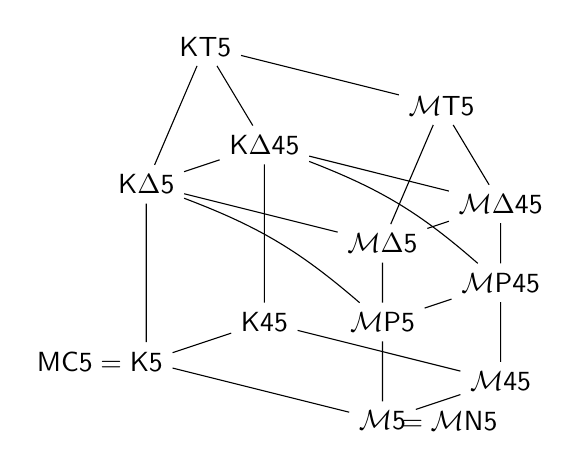
\begin{tikzpicture}
    \node (N5) at (0,0) {$\M\mathsf{5}$};
    \node (aux) at (.85,0) {$=\M\mathsf{N}\mathsf{5}$};
    \node (ND15) at (0,1.25) {$\M\mathsf{P}\mathsf{5}$};
    \node (ND25) at (0,2.25) {$\M\D\mathsf{5}$};
    \node (NT5) at (.75,4) {$\M\mathsf{T}\mathsf{5}$};
    \node (N45) at (1.5,.5) {$\M\mathsf{4}\mathsf{5}$};
    \node (ND145) at (1.5,1.75) {$\M\mathsf{P}\mathsf{4}\mathsf{5}$};
    \node (ND245) at (1.5,2.75) {$\M\D\mathsf{4}\mathsf{5}$};

    \draw (N5) -- (ND15) -- (ND25) -- (NT5) -- (ND245) -- (ND145) --
    (N45) -- (N5);
    \draw (ND15) -- (ND145);
    \draw (ND25) -- (ND245);

    \node (K5) at (-3,.75)  {$\mathsf{K}\mathsf{5}$};
    \node (aux2) at (-3.85,.75) {$\mathsf{MC5} = $};
    \node (KD5) at (-3,3) {$\mathsf{K}\D\mathsf{5}$};
    \node (KT5) at (-2.25,4.75) {$\mathsf{K}\mathsf{T}\mathsf{5}$};
    \node (K45) at (-1.5,1.25) {$\mathsf{K}\mathsf{4}\mathsf{5}$};
    \node (KD45) at (-1.5,3.5) {$\mathsf{K}\D\mathsf{4}\mathsf{5}$};
    \draw (K5) -- (KD5) -- (KT5) -- (KD45) -- (K45) -- (K5);
    \draw (KD5) -- (KD45);

    \draw (NT5) -- (KT5);
    \draw (ND25) -- (KD5);
    \draw (ND245) -- (KD45);
    \draw (ND15) to [bend right=10] (KD5);
    \draw (ND145) to [bend right=10] (KD45);
    \draw (N5) -- (K5);
    \draw (N45) -- (K45);
  \end{tikzpicture}
  \end{center}
  \hrule
  \caption{The extensions of modal logic $\M\mathsf{5}$}
  \label{fig:ext-m5}
\end{figure}


\cyan{
Elaine -- TODO:
\begin{itemize}
\item See to which logics of the classical cube there is: semantics and decision procedure;
\item produce a compilation with definition of neighbourhood semantics, etc;
\item the rule 
$$\infer{\Box A \seq \Box B}{A\seq B}$$
should be captured by enforcing that $A\to B$ is a tautology implies $\Box A\to \Box B$ is a tautology;
\item Try to see if the constraints on the relations given by extensions can be captured in the same way as Kripke;
\item How many values? Sets of sets of values?
\item try to reach all the extensions of the monotone logic in the tesseract.
\end{itemize}}

\bibliographystyle{alpha}
\bibliography{references} 
\end{document}
